\documentclass[11pt]{article}

\usepackage{graphicx, epsfig}
\usepackage{amsmath, amssymb, latexsym}
\usepackage[english]{babel}
\usepackage{amssymb}   
%\usepackage{graphicx}
%\usepackage{float} 






% Make a larger page (shrink the margins)
%
\setlength{\textwidth}{6.7in}
\setlength{\textheight}{9.0in}
\setlength{\evensidemargin}{0.0in}
\setlength{\oddsidemargin}{0.0in}
\topmargin -0.5in
\footskip 0.5in



\title{Progress Report}
\author{Eric}
\begin{document}
\maketitle
\medskip
\section{NORSTAR}
\hspace{0.5cm}

This week I again focused almost exclusively on programming with IDL. Initially looked at the script given to us by our supervisor that plotted the position of a star over a day for any known coordinates on earth, (example\_geo\_aim\_astro.pro). Although it worked well I think there could be better methods for identifying stars. This is also the first week we looked at data. During Monday/Tuesday we looked at files from the NORSTAR. I spent a while just getting familiarity with how IDL reads in files.  I created a code that easily lets you view the entire nights worth of data, or individual chunks easily. Looking at an entire night makes it difficult to see stars, especially if there are planets or the moon saturating the photometer. A little trial and error with the plotting methods gave me a good idea of what tends to produce useful data. The code itself is not too computationally intensive and it is not difficult to burn though an entire night's worth of data an hour at a time to spot something of interest.

\begin{figure}[t!]
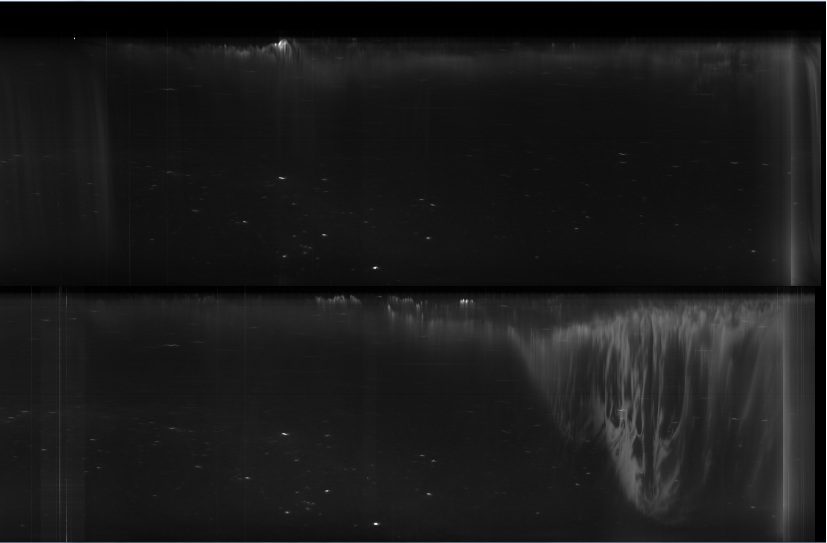
\includegraphics[scale=0.8]{keograms.jpg}
\caption{Keogram's from Gillam Manitoba's Themis site. Top keogram is from January 3rd 2011 while the bottom is January 1st 2011}
\end{figure}

\section{THEMIS}

 I transferred the data off of the Volume 1 drive, all 53 gigs worth. Specifically the stream2 data, which includes the first three days of data from all of the THEMIS sites. The code given produces an all sky video about 30 seconds long for the entire nights data. However, the latter part of the week was spent making keograms of this data in the hopes of spotting stars. This was accomplished (see figure 1)  and I now have a code that can easily compare the keograms of two different nights of data. A couple issues, the read file does take some time to run its course, and so cycling through hordes of files takes time.As well, identifying the stars in the pictures is more than a trivial problem. Although the Sky Calc should give us a very good idea of what stars will be passing through the line of sight, I have yet to come up with a quick and easy method for identifying the stars.  This is something I will spend some time on next week. However, it might just be a matter of working through Sky Calc to identify the correct stars we will need for absolute flux calibrations.  I was also to produce a code that takes a vertical profile of individual stars. From this profile I was able to get a polynomial and gaussian point spread function (PSF). However, in one sample star the full width half max of the star was approximately 1.01 pixels. As discussed above I was unable to find which star I was looking at, but as most stars tend to correspond to a pixel this gives me some hope that the optics are not distorting individual point sources (stars) too much. 




\section{Future Considerations}

Next week I really want to be able to identify stars from the THEMIS images with absolute certainty. Compare the PSF's from stars of different sizes/brightness/declinations. As well, I was never able to account for the gaps in the keograms successfully on a general code, so I need to do some touch ups to a couple of my codes. This hopefully will also help in identifying specific stars as well.





\end{document}
\end{article}